\documentclass[a4paper,12pt]{article}

%настройка кодировки
\usepackage[T2A]{fontenc}
\usepackage[utf8]{inputenc}
\usepackage[english,russian]{babel}
%основные библиотеки
\usepackage{amsmath, amsfonts, amssymb, amsthm, mathtools}

\usepackage{indentfirst}
\usepackage{icomma}
\usepackage{hyperref}
\usepackage{soulutf8}

\usepackage{multicol}
\usepackage{multirow}
\usepackage{hhline}
\usepackage{graphicx}
\usepackage{wrapfig}

\usepackage{geometry}
\geometry{top=25mm}
\geometry{bottom=30mm}
\geometry{left=20mm}
\geometry{right=20mm}

\renewcommand{\phi}{\varphi}
\renewcommand{\epsilon}{\varepsilon}

\title{Лабораторная работа \linebreak \textbf{Расход затопленной струи}}
\author{
    Фёдоров Марк\\
    \and
    Черней Кирилл\\
    \and
    Ерёмин Константин
}
\date{}

\begin{document}
    \begin{titlepage}
        \maketitle
        \vspace{-1.5cm}
        \begin{center}
            {\Large Б03-204}\\
            \vspace{1cm}
            \date{Ноябрь 2022}
        \end{center}
    \end{titlepage}

    \section{Введение}
        \textbf{Цель работы:} Рассчитать расход осесимметричной затопленной струи в различных сечениях и сделать вывод, 
            как он изменяется в зависимости от расстояния до сопла и почему.
        
        \textbf{Оборудование:} Компьютер, АЦП, датчик давления, трубка Пито и шаговой двигатель.

        \subsection*{Теоретическое описание}
            В данной лабораторной работе изучается затопленная струя. Потоки жидкости или газа, не имеющие твердых границ, называются соответственно жидкими или газовыми струями. Струи классифицируются по ряду признаков. Прежде всего различают затопленные и незатопленные струи. Если фазовое состояние истекающей жидкости отличается от фазового состояния окружающей среды (например, истечение воды в воздушное пространство), то такая струя называется незатопленной. Незатопленная жидкая струя движется в газовом пространстве, например, в воздухе. Если твёрдые стенки не оказывают влияния на течение, то такие течения называются свободными. В данной работе как раз исследуется свободная затопленная струя. Течение в затопленной струе можно разбить на несколько участков, находящихся на различном расстоянии от отверстия, из которого истекает поток. Границей является поверхность раздела, отделяющая саму струю от окружающей ее жидкости. Границей струи считают точки, в которых отношение скорости к скорости на оси имеет некоторое фиксированное значение. Поверхность струи по границам может быть «взрыхленной». На границе струи с окружающей неподвижной жидкостью происходит перемешивание между струей и окружающей жидкостью из-за эффекта вязкости и явления диффузии (броуновское движение) в ламинарном течении или интенсивных пульсаций скорости при турбулентном течении. Перемешивание приводит к тому, что между струей и окружающей средой происходит обмен количеством движения, струя подтормаживается, расширяется и одновременно увлекает с собой часть «внешней» жидкости. Вследствие этих эффектов расход струи увеличивается. Давление по длине струи сохраняется постоянным и равным давлению в окружающем пространстве. Количество движения струи по длине может меняться только из-за создающихся внешних вихрей и практически не изменяется. Визуальное представление струи можно увидеть на рисунках \ref{fig:structure} и \ref{fig:profile}.

            \begin{figure}[h]
                \centering
                \begin{minipage}{0.6\textwidth}
                    \centering
                    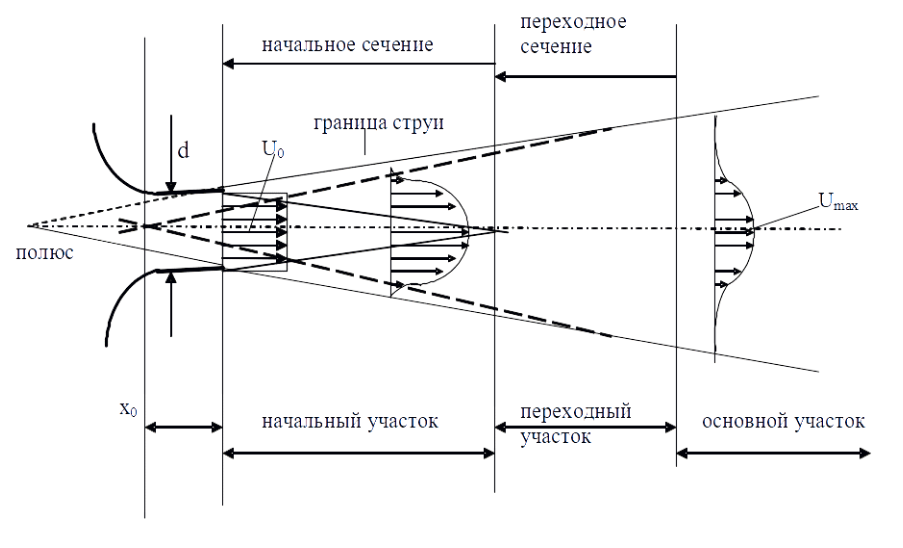
\includegraphics[width=0.9\linewidth]{structure}
                    \caption{Структура струи}
                    \label{fig:structure}
                \end{minipage}\hfill
                \begin{minipage}{0.4\textwidth}
                    \centering
                    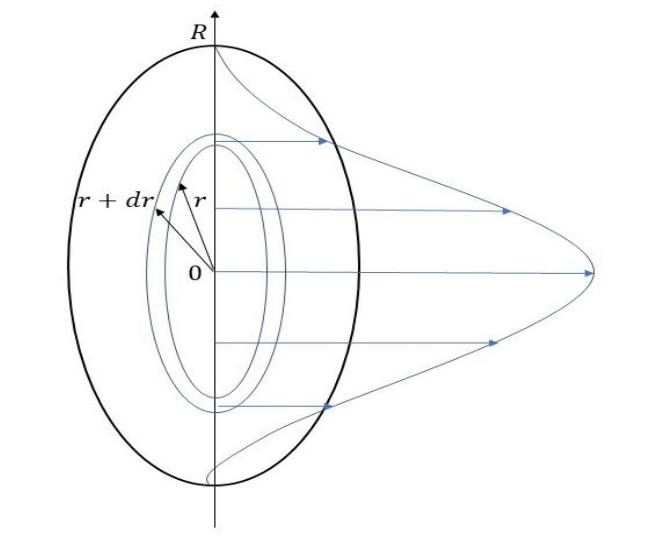
\includegraphics[width=0.9\linewidth]{profile}
                    \caption{Схематическое изображение профиля скорости в струе}
                    \label{fig:profile}
                \end{minipage}
            \end{figure}

            \newpage

            \begin{wrapfigure}{h}{0.4\textwidth}
                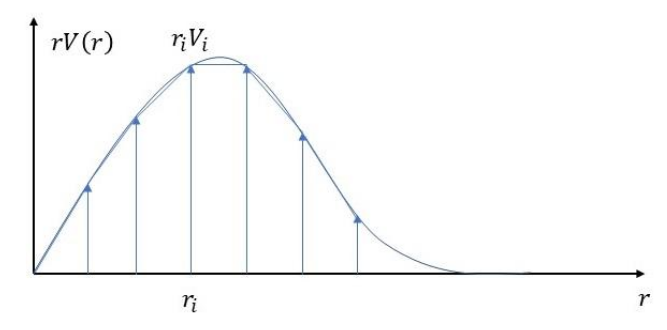
\includegraphics[width=0.38\textwidth]{data_example}
                \caption{Зависимость полученных результатов от расстояния до оси}
                \label{fig:data}
            \end{wrapfigure}
            Для описания струи вводится понятие расхода --- количество вещества, переместившегося через какую-либо поверхность. Расход может быть найден по формуле:
            \begin{equation}
                \label{eq:expence}
                Q_m = \int_0^R \rho 2\pi rV(r)dr
            \end{equation}

            В результате эксперимента и обработки будет определена скорость в отдельных точках, и, соответственно, произведение скорости на координату (радиус). Схематически это показано на рисунке \ref{fig:data}. В данном случае искомым расходом является площадь под графиком. Так как измерения проведены в конечном числе точек, то приближенно площадь можно определить, как сумму площадей трапеций, то есть по формуле:
            \begin{equation}
                \label{eq:final_expence}
                Q = 2\pi \sum_{i=0}^N 0.5\left(r_iV_i+r_{i+1}V{i+1}\right)\left(r_{i+1} - r_i\right)
            \end{equation}

            Уравнение Бернулли:
            \begin{equation}
                \label{eq:bernoulli}
                P + \frac{\rho V^2}{2} = P_0
            \end{equation}
            Второе слагаемое в левой части формулы называется динамическим напором, давление $P$ "--- это давление воздуха в текущей точке, а давление $P_0$ называется давлением торможения. Физический смысл давления торможения состоит в том, что при адиабатическом торможении газа давление возрастет до величины $P_0$. Давление $P$ "--- давление в струе, которое примерно равно давлению вне струи.
    
        \subsection*{Описание установки}
            На рисунке \ref{fig:setting} представлено используемое в работе оборудование. Основными элементами установки являются сопло, установка с шаговым двигателем, позволяющим перемещать трубку Пито перпендикулярно потоку газа, компьютер, датчик давления с АЦП. Также используется цифровой манометр для калибровки давления.
            
            \begin{figure}
                \centering
                \includegraphics[width=0.8\textwidth]{setting}
                \caption{Экспериментальная установка}
                \label{fig:setting}
            \end{figure}

            В момент запуска программы на компьютере предполагается, что будет подаваться сигнал на исполнительное устройство, заставляя трубку Пито переместиться вдоль струи на нужное расстояние, затем программой будет считано подряд несколько показаний датчика давления, вычислена средняя величина и прозведена запись в файл. На следующем шаге описанная последовательность действий должна быть повторена. Таким образом можно провести все необходимые измерения вдоль струи.

    \section{Ход работы}
        Перед началом работы было проведено знакомство с оборудованием и методами работы с ним: была просмотрена видео-инструкция по работе с внешним АЦП \emph{SPI}, были изучены функции из файлов \emph{jetFunctions.py} и \emph{jetMover.py} стартового набора.

        \subsection*{Калибровка}
            Также была проведена калибровка шагового двигателя и манометра.
            
            Для калибровки давления получены следующие величины: 
            \begin{itemize}
                \item показания АЦП при выключенном вентиляторе
                \item давление в струе (измерения цифровым манометром с трубкой Пито) при включённом вентиляторе
                \item показания АЦП при измеренном манометром давлении
            \end{itemize}
            
            Калибровка двигателя заключалась в получении количества шагов на известном расстоянии.
        
        \subsection*{Измерения}
            Измерения проводились следующим образом: трубка Пито устанавливалась напротив сопла вентилятора, а затем исполнялась программа.Трубка с помощью установки с шаговым двигателем передвигалась на 200 условных единиц ($\approx 11$ мм) в одну сторону, после чего проходила 400 единиц в другую. Один шаг составлял 10 единиц ($\approx 0.6$ мм), а после каждого шага брались показания 1000 значений АЦП и усреднённое значение записывалось в файл. После подобной серии измерений вентилятор вручную отодвигался от трубки Пито и измерения проводились снова. Таким образом были собраны данные на расстояниях от 0 до 100 миллиметров от сопла вентилятора с шагом 10 мм.

        \subsection*{Обработка}
            В первую очередь были найдены калибровочные коэффициенты расстояния и давления. Результаты калибровки представлены графически на рисунке \ref{fig:calibration}, численные значения: в одном шаге АЦП "--- 0.1596 Па, в одном шаге двигателя "--- 0.0056 cм.
            
            \begin{figure}[h]
                \centering
                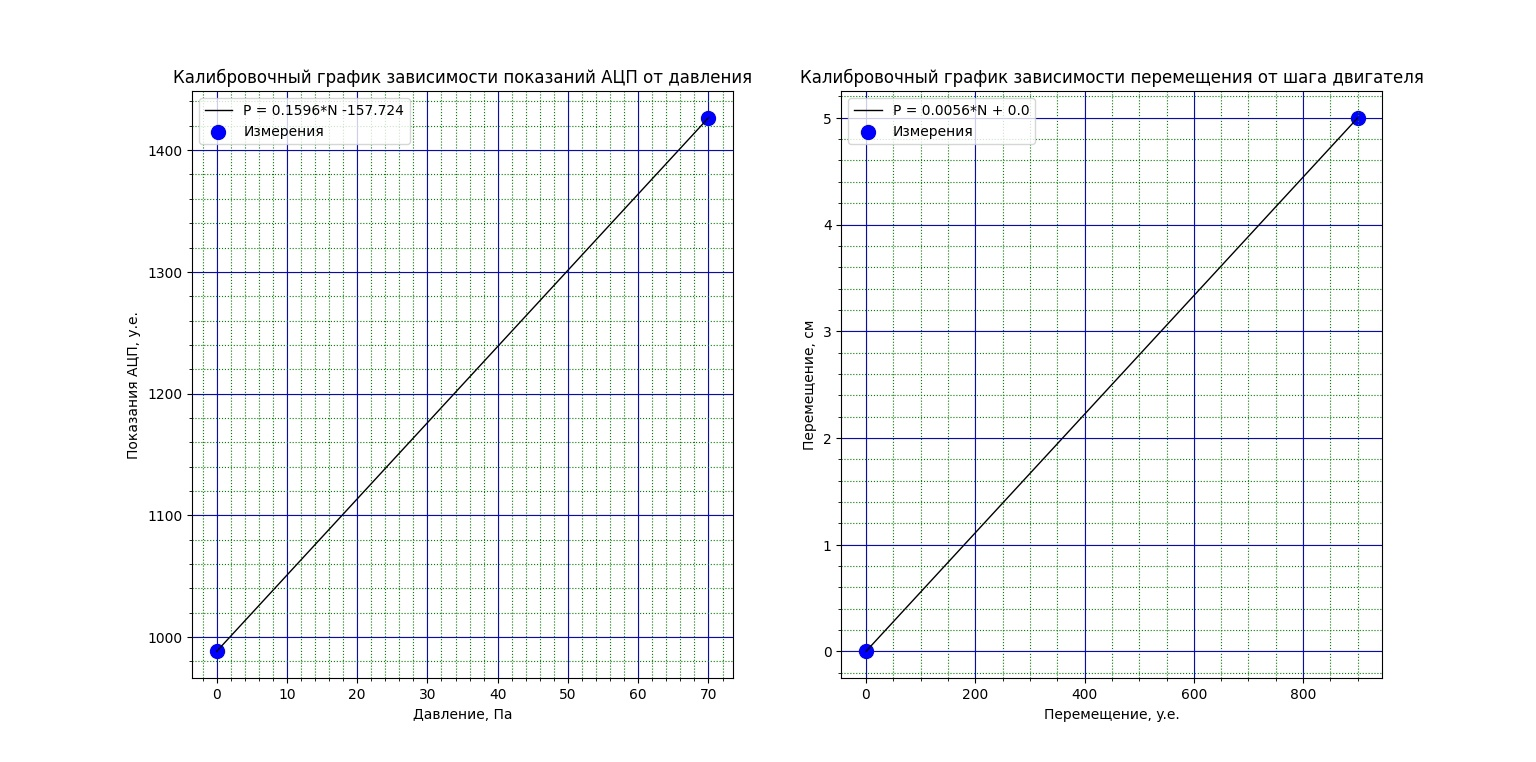
\includegraphics[width=\textwidth]{calibration.jpg}
                \caption{Результаты калибровки}
                \label{fig:calibration}
            \end{figure}

            Далее записанные в файлы значения давления были пересчитаны по формуле Бернулли \ref{eq:bernoulli} в скорости. С этими данными, предварительно центрированными по максимуму, был построен график (рисунок \ref{fig:expence}). На этом же графики представлены результаты расчётов расхода в каждом из сечений с помощью формулы \ref{eq:final_expence}.

            \begin{figure}[h!]
                \centering
                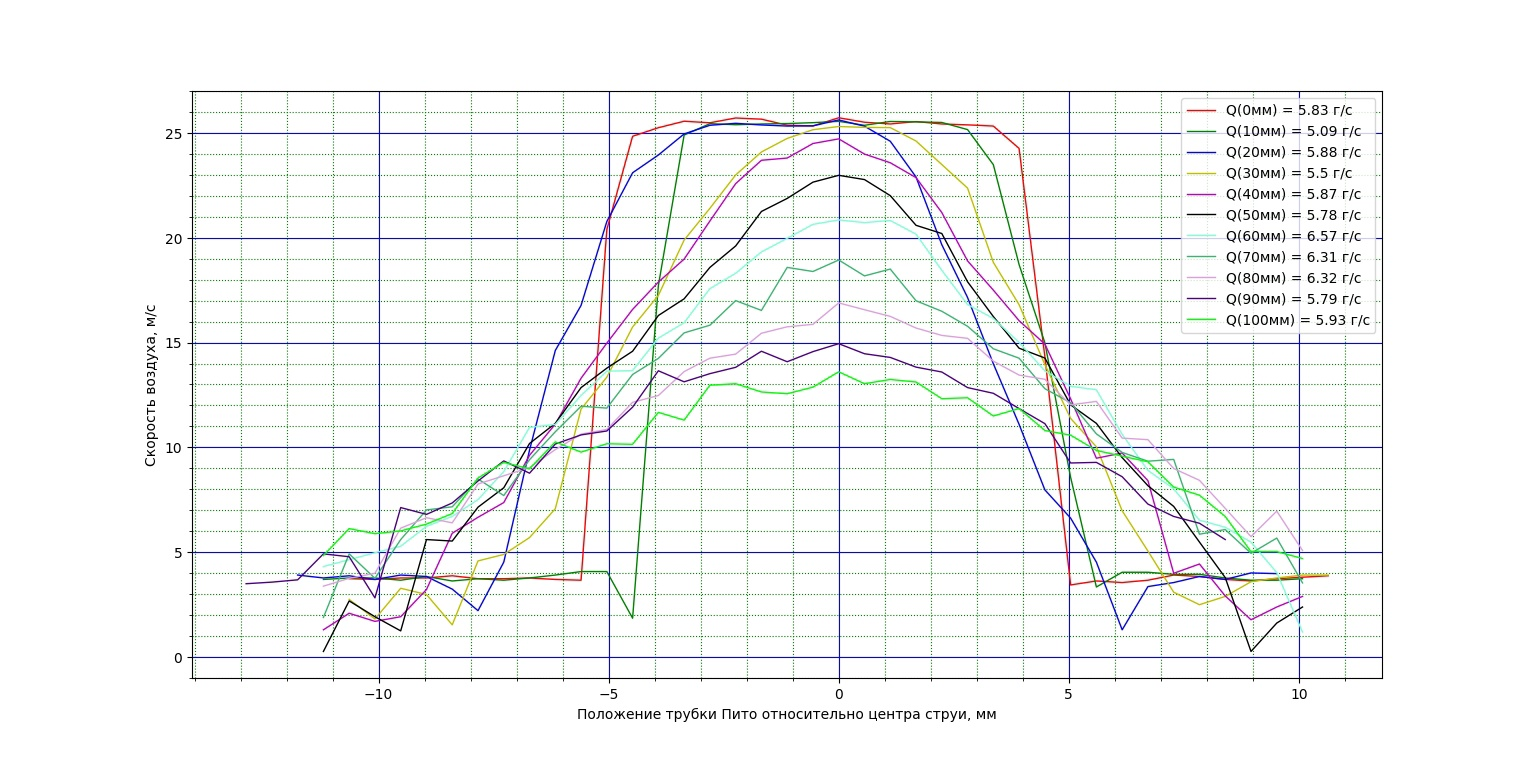
\includegraphics[width=\textwidth]{expence.jpg}
                \caption{График скоростей с рассчитанными расходами}
                \label{fig:expence}
            \end{figure}

%Построить график зависимости расхода от расстояния до сопла - 1 балл

    \section{Вывод}
        В ходе работы были получены скорости струи в зависимости от расстояния до её оси, построены соответствующие графики, хорошо описывающие теорию. Для каждого удаления был рассчитан расход, однако его поведение не совпало с теоретически предсказанным.

\end{document}
